\documentclass[11pt]{article} 
\usepackage[utf8]{inputenc} 
\usepackage{geometry} 
\geometry{a4paper} 
\usepackage{graphicx} 
\graphicspath{ {./Images/} }
\usepackage{booktabs} 
\usepackage{array} 
\usepackage{paralist} 
\usepackage{verbatim} 
\usepackage{subfig} 
\usepackage{tikz}
\usepackage{hyperref}
\usetikzlibrary{shapes,arrows}
\usepackage{verbatim}
\usepackage{fancyhdr} 
\usepackage{tcolorbox}
\usepackage{xcolor}
\usepackage{fancyvrb}
\usepackage{emoji}
\usepackage[toc,page]{appendix}
\usepackage{amsmath}
\DeclareMathOperator*{\argmax}{arg\,max}
\DeclareMathOperator*{\argmin}{arg\,min}
\pagestyle{fancy} 
\renewcommand{\headrulewidth}{0pt} 
\lhead{}\chead{}\rhead{}
\lfoot{}\cfoot{\thepage}\rfoot{}
\usepackage{textcomp}
\usetikzlibrary{shapes,arrows}
\usepackage{sectsty}
\allsectionsfont{\sffamily\mdseries\upshape} 
\usepackage[nottoc,notlof,notlot]{tocbibind} 
\usepackage[titles,subfigure]{tocloft}
\renewcommand{\cftsecfont}{\rmfamily\mdseries\upshape}
\renewcommand{\cftsecpagefont}{\rmfamily\mdseries\upshape} 

\definecolor{darkgreen}{HTML}{00AA00}
\definecolor{myred}{rgb}{0.8, 0.0, 0.0}
\definecolor{ao}{rgb}{0.0, 0.5, 0.0}

\newcommand{\inBlue}[1]{\textcolor{blue}{#1}}
\newcommand{\inRed}[1]{\textcolor{myred}{#1}}
\newcommand{\inGreen}[1]{\textcolor{ao}{#1}}


\large\title{Physical Attacks on Secure Systems (NWI-IMC068)}
\author{Tutorial 4: Leakage assessment}
\date{Omid Bazangani (omid.bazangani@ru.nl)} % Activate to display a given date or no date (if empty),
         % otherwise the current date is printed 

\begin{document}
\setemojifont{TwemojiMozilla}
\maketitle
\noindent \textbf{Goals:} After completing this tutorial successfully, you should understand how to conduct a TVLA test for a leakage assessment, choose a fix-set and random-set, record the dataset, and how interpret the result.   \\\\

\noindent \textbf{Before you start:} To complete this tutorial, your teacher will provide you with a package that contains the Chipwhisper-lite board. You will collect the traces with Chipwhisperer as you did in previous tutorials.


\section{Test Vector Leakage Assessment (TVLA)}
Leakage assessment can be done independently from any specific intermediate values and only depends on key or input. This test is called the Non-Specific TVLA test. In contrast, Specific TVLA evaluates a specific intermediate value. You can find more information \href{https://www.rambus.com/wp-content/uploads/2015/08/TVLA-DTR-with-AES.pdf} {here}.
This tutorial will apply a Non-Specific TVLA test on the \href{https://github.com/kokke/tiny-AES-c}{TinyAES} implementation running on an ARM Cortex-M3 microcontroller~(\texttt{STM32F303}) using the ChipWhisperer framework. In this assessment, we investigate if an adversary can learn about the key by analyzing the power traces for fixed data compared to random data. 

\subsection{Test Requirments}
Using the ChipWhisperer framework gives you access to an implemented TinyAES firmware ready to run on the target. A Jupyter notebook file~(\texttt{.ipynb}) is provided to guide you to conduct the test step by step. You can download the file from \href{https://mega.nz/file/pggmkDqK#Bh2cE_imutKkWBbRUpEl8mkgE8pxKxfeaInNOgVU_yE} {the link}. After downloading the file, you need to place it in the ChipWhisperer directory. For example, in Windows, it can be like: "\path{C:\Users\USER\ChipWhisperer_xx\cw\home\portable\chipwhisperer\jupyter\experiments}." \footnote{In Linux or MAC, the path can be different. You must put the notebook file in the correct directory based on the operating system.}\\\\ This file consists of five Steps as follows. 
\begin{enumerate}
    \item Configure platform and crypto algorithm and compile the firmware 
    \item Configure and connect to the ChipWhisperer
    \item Configure the programmer and flash the target
    \item Trace record and dataset creation~( \inRed {needs to be completed by you})
    \item Apply the TVLA test~( \inRed{needs to be completed by you})
\end{enumerate}

\subsection{Step1:}
In this step, we will select the firmware that we need~(TinyAES), the target board~(CWLITEARM), and the ChipWhisperer scope. \\  

\begin{small} 
\begin{tcolorbox}
\begin{Verbatim}[commandchars=\\\{\}]
\textcolor{orange}{# Config Platform, Crypto Algorithm and Scope }

SCOPETYPE \textcolor{purple}{=} \textcolor{red}{"OPENADC"}
PLATFORM  \textcolor{purple}{=} \textcolor{red}{"CWLITEARM"}
CRYPTO_TARGET  \textcolor{purple}{=} \textcolor{red}{"TINYAES128C"}
\end{Verbatim}
\end{tcolorbox}
\end{small} 


\noindent The following cell of the jupyter notebook file is responsible for compiling the code and making the firmware.\footnote{The provided bash script is a Windows-compatible command. You must replace it with proper commands based on your OS.}\\


\begin{small} 
\begin{tcolorbox}
\begin{Verbatim}[commandchars=\\\{\}]
\textcolor{orange}{# Compile the firmware for the introduced target }

%%bash -s "$PLATFORM" "$CRYPTO_TARGET" 
\textcolor{darkgreen}{cd}  \textcolor{black}{../../hardware/victims/firmware/simpleserial-aes}
\textcolor{darkgreen}{make} \textcolor{blue}{PLATFORM}\textcolor{purple}{=}\textcolor{blue}{$1} \textcolor{blue}{CRYPTO_TARGET}\textcolor{purple}{=}\textcolor{blue}{$2}
\end{Verbatim}
\end{tcolorbox}
\end{small} 


\subsection{Step2:}
This step checks if the ChipWhisperer is connected to the USB port, and then it Would connect to it. Otherwise, you better check the USB port and make sure the driver of your ChipWhisperer is appropriately installed.  

\begin{small} 
\begin{tcolorbox}
\begin{Verbatim}[commandchars=\\\{\}]
\textcolor{darkgreen}{import} chipwhisperer \textcolor{darkgreen}{as} cw
\textcolor{darkgreen}{import} usb

\textcolor{darkgreen}{try}:
    \textcolor{darkgreen}{try}:
        \textcolor{darkgreen}{if not}: scope.connectStatus:
            scope.con()
    \textcolor{darkgreen}{except}: NameError:
        scope \textcolor{purple}{=} cw.scope()

    try:
        if SS_VER \textcolor{purple}{==} \textcolor{red}{"SS_VER_2_0"}:
            target_type \textcolor{purple}{=} cw.targets.SimpleSerial2
        else:
            target_type \textcolor{purple}{=} cw.targets.SimpleSerial
    except:
        SS_VER\textcolor{purple}{=}\textcolor{red}{"SS_VER_1_1"}
        target_type \textcolor{purple}{=} cw.targets.SimpleSerial

    try:
        target \textcolor{purple}{=} cw.target(scope, target_type)
    except IOError:
        print(\textcolor{red}{"INFO: Caught exception on reconnecting to target attempting} 
              \textcolor{red}{ to reconnect to scope first."})
        print(\textcolor{red}{"INFO: This is a work-around when USB has died without Python} 
              \textcolor{red}{knowing. Ignore errors above this line."})
        scope \textcolor{purple}{=} cw.scope()
        target \textcolor{purple}{=} cw.target(scope, target_type)
except:
    if usb.__version__ \textcolor{purple}{<} '1.1.0':
        print(\textcolor{red}{"-----------------------------------"})
        print("\textcolor{red}{Unable to connect to chipwhisperer. pyusb {} detected}
        \textcolor{red}{(>= 1.1.0 required)"}.format(usb.__version))
        print(\textcolor{red}{"-----------------------------------"})
    raise

print("\textcolor{red}{INFO: Found ChipWhisperer"})

\end{Verbatim}
\end{tcolorbox}
\end{small} 

\subsection{Step3:}
Before starting trace collection, you must program the chip with the compiled firmware.  
The next two cells show how the ChipWhisperer configs the built-in programmer, and the third cell defines the firmware path and follows which it programs the chip using \texttt{cw.program\_target()} command. 


\begin{small} 
\begin{tcolorbox}
\begin{Verbatim}[commandchars=\\\{\}]
\textcolor{orange}{# Choosing the proper programmer based on the platform }

\textcolor{darkgreen}{if} \textcolor{red}{"STM"} \textcolor{darkgreen}{in} PLATFORM \textcolor{darkgreen}{or} PLATFORM \textcolor{purple}{==} \textcolor{red}{"CWLITEARM"} \textcolor{darkgreen}{or} PLATFORM \textcolor{purple}{==} \textcolor{red}{"CWNANO"}:
    prog \textcolor{purple}{=} cw.programmers.STM32FProgrammer
\textcolor{darkgreen}{elif} PLATFORM \textcolor{purple}{==} \textcolor{red}{"CW303"} \textcolor{darkgreen}{or} PLATFORM \textcolor{purple}{==} \textcolor{red}{"CWLITEXMEGA"}:
    prog \textcolor{purple}{=} cw.programmers.XMEGAProgrammer
\textcolor{darkgreen}{else}:
    prog \textcolor{purple}{=} \textcolor{darkgreen}{None}
\end{Verbatim}
\end{tcolorbox}
\end{small} 

\begin{small} 
\begin{tcolorbox}
\begin{Verbatim}[commandchars=\\\{\}]
\textcolor{orange}{# GPIO pin configuration act as the trigger signal for Oscope }

\textcolor{darkgreen}{import} time
time.sleep(\textcolor{darkgreen}{0.05})
scope.default_setup()
\textcolor{darkgreen}{def} reset_target(scope):
    \textcolor{darkgreen}{if} PLATFORM \textcolor{purple}{==} \textcolor{red}{"CW303"} \textcolor{darkgreen}{or} PLATFORM \textcolor{purple}{==} \textcolor{red}{"CWLITEXMEGA"}:
        scope.io.pdic \textcolor{purple}{=} \textcolor{red}{"low"}
        time.sleep(\textcolor{darkgreen}{0.1})
        scope.io.pdic \textcolor{purple}{=} \textcolor{red}{"high_z"}  \textcolor{orange}{#XMEGA doesn't like pdic driven high}
        time.sleep(\textcolor{darkgreen}{0.1})           \textcolor{orange}{#xmega needs more startup time}
    \textcolor{darkgreen}{else}:  
        scope.io.nrst \textcolor{purple}{=} \textcolor{red}{"low"}
        time.sleep(\textcolor{darkgreen}{0.05})
        scope.io.nrst \textcolor{purple}{=} \textcolor{red}{"high_z"}
        time.sleep(\textcolor{darkgreen}{0.05})
\end{Verbatim}
\end{tcolorbox}
\end{small} 

\begin{small} 
\begin{tcolorbox}
\begin{Verbatim}[commandchars=\\\{\}]
\textcolor{orange}{# program the chip with the compiled firmware }

fw_path \textcolor{purple}{=} \textcolor{red}{'../../hardware/victims/firmware/simpleserial-aes/}
           \textcolor{red}{simpleserial-aes-{}.hex'}.format(PLATFORM)
cw.program_target(scope, prog, fw_path)
\end{Verbatim}
\end{tcolorbox}
\end{small} 


\subsection{Step4:}
This section aims to capture a trace set to conduct a Non-Specific TVLA test on it. We need to capture a fixed and random dataset based on a fixed and random plain text fed to the target while the key is fixed~(Fig~\ref{fig:TVLA-Setup}). 

\begin{figure}[]
    \centering
    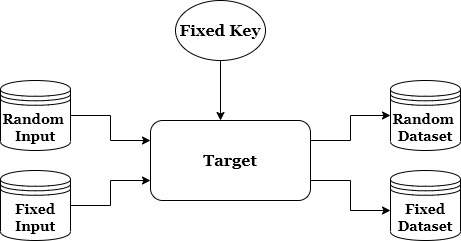
\includegraphics[scale=0.75]{TVLA-FI-Images/TVLA_setup.jpg}
    \caption{TVLA dataset construction}
    \label{fig:TVLA-Setup}
\end{figure}

\noindent Statistically, it's important how the fixed and random plain text and the fixed key are chosen, and there are specific rules for it. For the AES algorithm, it has been suggested to choose the fixed key~({$K_{Fixed}$}) as follows:

\begin{itemize}
    \item 0x0123456789abcdef123456789abcdef0 \inGreen{for AES‐128}
    \item 0x0123456789abcdef123456789abcdef023456789abcdef01 \inGreen{for AES‐192}
    \item 0x0123456789abcdef123456789abcdef023456789abcdef013456789abcdef012 \inGreen{for AES‐256} 

\end{itemize}


\noindent Setting the fixed key, for the fixed data datasets, perform n encryptions with the fixed plaintext~({$P_{Fixed}$}) set as follows: 

\begin{itemize}
    \item 0xda39a3ee5e6b4b0d3255bfef95601890 \inGreen{for AES‐128}
    \item 0xda39a3ee5e6b4b0d3255bfef95601888 \inGreen{for AES‐192}
    \item 0xda39a3ee5e6b4b0d3255bfef95601895 \inGreen{for AES‐256}
\end{itemize}

\noindent Constructing the random dataset needs a random set of plaintext~(\texttt{$P_{Rand}$} which is randomized by encryption of the key and previous plaintext as follows: 

\begin{itemize}
    \item $I_0$ = 0x00...0  \inGreen{(16 bytes of zeros)}
    \item $I_{j+1}$ = AES($K_{gen}$, $I_j$ ) for 0 $\leq$ j $< n$
\end{itemize}

Although in the ChipWhisperer framework, the required key and plaintexts are handled by \href{https://chipwhisperer.readthedocs.io/en/latest/capture-api.html#tvla-ttest}{AcqKeyTextPattern\_TVLATTest class}, You can find more information about it in a paper provided by Rambus Company \href{https://www.rambus.com/test-vector-leakage-assessment-tvla-derived-test-requirements-dtr-with-aes/}{here}. 

\noindent Having the fixed key and plaintext set raises the question of "in which order should the trace be collected?". The answer is, The two datasets should be recorded \inBlue{randomly interspersed} to avoid any \inRed{systematic bias} due to the order of collection. 
It means we must collect one fixed trace followed by a random trace, and so on~(~Fig\ref{fig:TVLA-Dataset}). You will see it would be done easily by using \texttt{AcqKeyTextPattern\_TVLATTest} class in the ChipWhisperer framework.

\begin{figure}[]
    \centering
    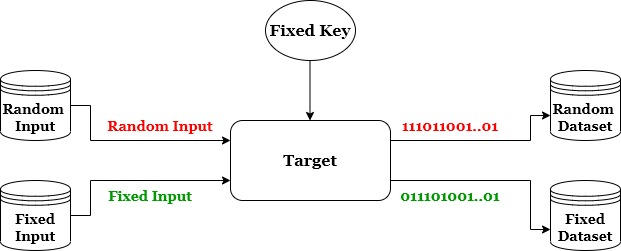
\includegraphics[scale=0.65]{TVLA-FI-Images/TVLA_dataset.jpg}
    \caption{TVLA dataset order}
    \label{fig:TVLA-Dataset}
\end{figure}

\noindent In order to construct the dataset, you need to complete the \texttt{Jupyter Notebook} code. It's as follows: 

\begin{small} 
\begin{tcolorbox}
\begin{Verbatim}[commandchars=\\\{\}]
\textcolor{orange}{ #Capture Traces }

\textcolor{darkgreen}{from} tqdm \textcolor{darkgreen}{import} trange
\textcolor{darkgreen}{import} numpy \textcolor{darkgreen}{as} np

N \textcolor{purple}{=} \textcolor{darkgreen}{10000}  \textcolor{orange}{# Number of traces (50% Fixed 50% Random)}
ktp \textcolor{purple}{=} cw.ktp.TVLATTest()
ktp.init(N)          \textcolor{orange}{# init with the number of traces you plan to}

traces \textcolor{purple}{=} []
Fix_text \textcolor{purple}{=} \textcolor{darkgreen}{bytearray}.fromhex(\textcolor{red}{"da39a3ee5e6b4b0d3255bfef95601890"})

Random_project \textcolor{purple}{=} cw.create_project(\textcolor{red}{"RandomSet.cwp"})
Fix_project \textcolor{purple}{=} cw.create_project(\textcolor{red}{"FixSet.cwp"})

\textcolor{darkgreen}{for} i \textcolor{darkgreen}{in} trange(N, desc\textcolor{purple}{=}\textcolor{red}{'Capturing traces'}):
    key, text \textcolor{purple}{=} ktp.next() \textcolor{orange}{# Select the Next key and plaintext}
   
    trace \textcolor{purple}{=} ...    \textcolor{orange}{#Code needs to be completed}
    
     \textcolor{orange}{#You need to append traces either in the Random or the Fixed project}
     \textcolor{orange}{based on their fed text!}
\end{Verbatim}
\end{tcolorbox}
\end{small} 

% cw.capture_trace(scope, target, text, key)
  
%     \textcolor{darkgreen}{if} trace \textcolor{darkgreen}{is None}:
%         \textcolor{darkgreen}{print}(\textcolor{red}{"error"})
%         \textcolor{darkgreen}{continue}
%     \textcolor{darkgreen}{if} text\textcolor{purple}{==}Fix_text:
%         Fix_project.traces.append(trace)
%     \textcolor{darkgreen}{else}:
%         Random_project.traces.append(trace)

\subsection{Step5:}
Having the required dataset for the test\footnote{Note: if you cannot capture traces using ChipWhisperer, You can download the provided dataset from this \href{https://mega.nz/folder/IoYxUIqC\#vTX_8ll83x7fx7IEx3OraQ}{link}. The provided dataset consists of two different power trace files in \texttt{.npy} format, one for fixed data and the other for random data.}, we can apply the TVLA test in Python using \textbf{ttest\_ind} function from \textbf{statistics library}. \\


\noindent \inGreen{ttest\_rslt}, \inGreen{pvalue\_rslt} = stats.ttest\_ind(Fixed\_dataset [ ][ ], Random\_dataset [ ][ ], equal\_var=False)\\
In order to use this function, you need to import \texttt{stats} from \texttt{scipy} library~(\inGreen{from} scipy \inGreen{import} stats).\\

\textbf{Some useful tips.}
\begin{itemize}
\item To find the samples which failed the test, compare \inBlue{ttest\_rslt} with the threshold \inBlue{($+/-4.5$)}. 
\item Argument \textbf{equal\_var} should be \inGreen{False} (to apply Welch's t-test). 
\item Do not forget about \inRed{the negative part} of the threshold value. 
\item Plot the result of the t-test. 
\end{itemize}

\noindent Considering the aforementioned tips, you must complete the following code in the Jupyter Notebook provided. 
\begin{small} 
\begin{tcolorbox}
\begin{Verbatim}[commandchars=\\\{\}]
\textcolor{orange}{#Apply TVLA test on the provided Dataset}

\textcolor{darkgreen}{from} scipy \textcolor{darkgreen}{import} stats
\textcolor{darkgreen}{import} matplotlib.pyplot \textcolor{darkgreen}{as} plt 
ttest_rslt, pvalue_rslt \textcolor{purple}{=} stats.ttest_ind(..., equal_var\textcolor{purple}{=}\textcolor{darkgreen}{False})
                          
\textcolor{orange}{#Code needs to be completed}
...

\textcolor{darkgreen}{print}(\textcolor{red}{f"Number of leaky points are: ..."})

\textcolor{orange}{#Plot the TVLA Graph}
plt.figure(figsize\textcolor{purple}{=}(\textcolor{darkgreen}{9}, \textcolor{darkgreen}{3}))
plt.plot(ttest_rslt)
plt.xlabel(\textcolor{red}{"Samples"})
plt.ylabel(\textcolor{red}{"t-test value: "})
plt.axhline(y\textcolor{purple}{=}\textcolor{darkgreen}{4.5}, color\textcolor{purple}{=}\textcolor{red}{'r'}, linestyle=\textcolor{red}{':'})
plt.axhline(y\textcolor{purple}{=}-\textcolor{darkgreen}{4.5}, color\textcolor{purple}{=}\textcolor{red}{'r'}, linestyle=\textcolor{red}{':'})
plt.ylim((-\textcolor{darkgreen}{20}, \textcolor{darkgreen}{20}))
plt.xlim((\textcolor{darkgreen}{0}, \textcolor{darkgreen}{len}(ttest_rslt)))
plt.title(\textcolor{red}{'TinyAES Implementation'})
plt.savefig(\textcolor{red}{"TinyAes_TVLA.jpg"})
plt.tight_layout()

\end{Verbatim}
\end{tcolorbox}
\end{small} 
%Fix_project.waves[:][:],
                          % Random_project.waves[:][:]
\newpage

\section{Questions}
After successfully conducting the test, you can challenge yourself by answering the following questions. 

 \begin{enumerate}
        \item How can you interpret the TVLA graph?
        \item How many leaky points did you find? 
        \item Is there any relation between the number of traces and the number of leaky points?
        \item Can you think of any countermeasure against the TVLA test?
        \item How do you interpret a high-value compared to a low-value for test results?
        \item Can you explain how we can return to the software from power trace to pinpoint the cause of leakage?
        
        
    \end{enumerate}

\end{document}